% Fonte do fluxograma PRISMA 2020 (Figura do Capítulo 3).
% COMO ATUALIZAR: edite os números abaixo; no Overleaf, menu > "Main document" > escolha este arquivo,
% clique em Recompile, baixe o PDF gerado e substitua figures/prisma2020.pdf. Depois volte o "Main document" para main.tex.
% (Pré-compilado em PDF para reduzir o tempo de compilação do main.tex no plano gratuito do Overleaf.)
% Números: busca de 21/11/2026; decisão de cada registro em prisma/triagem_prisma.csv.
\documentclass[border=4pt]{standalone}
\usepackage[T1]{fontenc}
\usepackage[utf8]{inputenc}
\usepackage{xcolor}
\usepackage{tikz}
\usetikzlibrary{positioning,arrows.meta,calc}
\newcommand{\validar}[1]{{\color{red}#1}}
\begin{document}
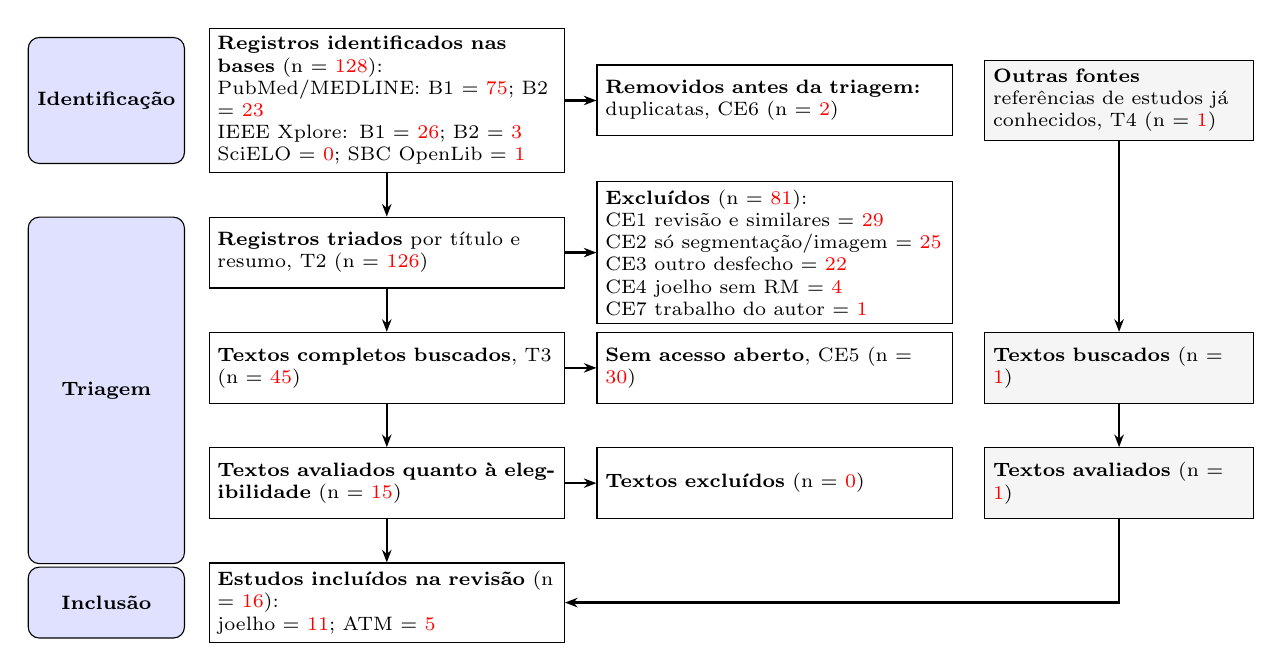
\begin{tikzpicture}[
  font=\scriptsize,
  caixa/.style={draw, rectangle, align=left, text width=4.3cm, inner sep=3pt, minimum height=0.9cm},
  lateral/.style={draw, rectangle, align=left, text width=4.3cm, inner sep=3pt, minimum height=0.9cm},
  outra/.style={draw, rectangle, align=left, text width=3.2cm, inner sep=3pt, minimum height=0.9cm, fill=gray!8},
  etapa/.style={draw, rectangle, rounded corners, fill=blue!12, text width=1.75cm, align=center, font=\scriptsize\bfseries},
  seta/.style={-{Stealth[length=1.6mm]}, thick}]
\node[caixa] (id) {\textbf{Registros identificados nas bases} (n = \validar{128}):\\
  PubMed/MEDLINE: B1 = \validar{75}; B2 = \validar{23}\\
  IEEE Xplore: B1 = \validar{26}; B2 = \validar{3}\\
  SciELO = \validar{0}; SBC OpenLib = \validar{1}};
\node[lateral, right=0.4cm of id] (dup) {\textbf{Removidos antes da triagem:}\\ duplicatas, CE6 (n = \validar{2})};
\node[outra, right=0.4cm of dup] (oid) {\textbf{Outras fontes}\\ referências de estudos já conhecidos, T4 (n = \validar{1})};

\node[caixa, below=0.55cm of id] (tri) {\textbf{Registros triados} por título e resumo, T2 (n = \validar{126})};
\node[lateral, right=0.4cm of tri] (exc1) {\textbf{Excluídos} (n = \validar{81}):\\
  CE1 revisão e similares = \validar{29}\\ CE2 só segmentação/imagem = \validar{25}\\ CE3 outro desfecho = \validar{22}\\ CE4 joelho sem RM = \validar{4}\\ CE7 trabalho do autor = \validar{1}};

\node[caixa, below=0.55cm of tri] (busca) {\textbf{Textos completos buscados}, T3 (n = \validar{45})};
\node[lateral, right=0.4cm of busca] (nao) {\textbf{Sem acesso aberto}, CE5 (n = \validar{30})};
\node[outra, right=0.4cm of nao] (obusca) {\textbf{Textos buscados} (n = \validar{1})};

\node[caixa, below=0.55cm of busca] (eleg) {\textbf{Textos avaliados quanto à elegibilidade} (n = \validar{15})};
\node[lateral, right=0.4cm of eleg] (exc2) {\textbf{Textos excluídos} (n = \validar{0})};
\node[outra, right=0.4cm of exc2] (oeleg) {\textbf{Textos avaliados} (n = \validar{1})};

\node[caixa, below=0.55cm of eleg] (inc) {\textbf{Estudos incluídos na revisão} (n = \validar{16}):\\ joelho = \validar{11}; ATM = \validar{5}};

\draw[seta] (id) -- (tri); \draw[seta] (tri) -- (busca); \draw[seta] (busca) -- (eleg); \draw[seta] (eleg) -- (inc);
\draw[seta] (id) -- (dup); \draw[seta] (tri) -- (exc1); \draw[seta] (busca) -- (nao); \draw[seta] (eleg) -- (exc2);
\draw[seta] (oid) -- (obusca); \draw[seta] (obusca) -- (oeleg);
\draw[seta] (oeleg.south) |- (inc.east);

\node[etapa, left=0.3cm of id, minimum height=1.6cm] {Identificação};
\node[etapa, minimum height=4.4cm, anchor=north east] at ($(tri.north west)+(-0.3cm,0)$) {Triagem};
\node[etapa, left=0.3cm of inc, minimum height=0.9cm] {Inclusão};
\end{tikzpicture}
\end{document}
